\subsection{Übertragen der Config Files mittels USB}
Um dem Programm die neuesten Konfigurationsdateien zu übergeben, steckt man beim Bootvorgang des Raspberry Pi einen Datenträger (\zB USB-Stick) an. Auf dem Datenträger muss im Root-Verzeichnis (\textasciitilde) ein Verzeichnis namens \enquote{RLT\_Config} sein. Wenn dieses Verzeichnis und alle nötigen Konfigurationsdateien darin vorhanden sind, werden diese in das Documents Verzeichnis des Raspberry Pi kopiert. \newline Folgendes Aktivitätsdiagramm verdeutlicht diesen Vorgang. (Siehe Abb.~\ref{fig:config_ubertragen_activity}):
\begin{figure}[H]
	\centering
	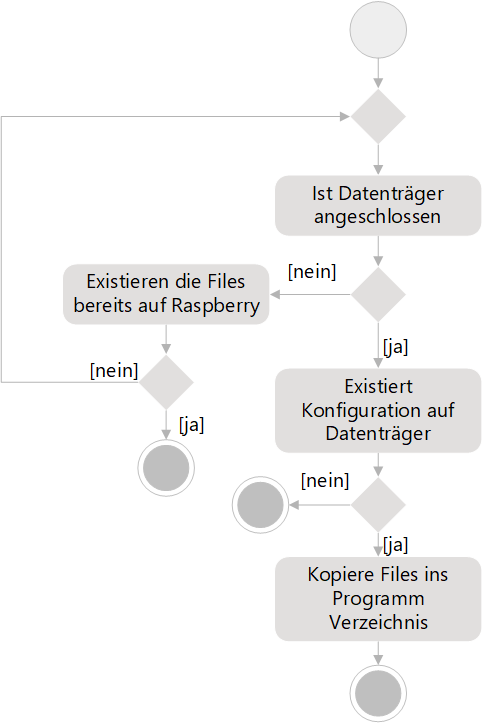
\includegraphics[width=0.4\linewidth]{Bilder/config_ubertragen_activity_diagram}
	\caption{Übertragen der Konfigurationsdateien}
	\label{fig:config_ubertragen_activity}
\end{figure}

Der gesamte Ablauf passiert in der \enquote{usb\_routine} Funktion. Diese Funktion liefert einen Fehlercode zurück, der daraufhin in einer Verzweigung abgefragt wird. Wenn ein Fehler beim Übertragen auftritt, terminiert das Programm. Ansonsten fährt das Programm fort.
\begin{pythoncode}
if __name__ == "__main__":
	copy_error = usb_detection.usb_routine()
	if copy_error:
		exit
	all_pages = modbus.load_config()
	global app
	app = App(all_pages)
	setup_buttons()
	modbus.data_threading(app)
	app.mainloop()	
\end{pythoncode}

In der \enquote{usb\_routine} Funktion wird die \enquote{copy\_from\_usb} Funktion aufgerufen. Diese gibt einen Statuscode zurück. Die \enquote{start\_window} Funktion erstellt ein neues customtkinter Fenster, in dem dann als Parameter angegebene Zeichenkette angezeigt wird. Das Fenster bleibt für sieben Sekunden offen, bevor es wieder geschlossen wird und die Ausführung fortfährt. Die \enquote{usb\_routine} Funktion dient als Zwischenschritt, damit der Benutzer eine Rückmeldung bekommt, ob die Konfigurationsdateien erfolgreich kopiert wurden oder keine Änderung vorgenommen wird.

\begin{pythoncode}
def usb_routine():
	copy_status = copy_from_usb()
	if copy_status == -1:
		return True # Kein Fehler
	elif copy_status == 0:
		start_window("Config Dateien wurden kopiert. Entferne nun den USB")   
	elif copy_status == 1: 
		start_window("Kein USB-Stick gefunden und Config bereits vorhanden")  
	return False # Fehler
\end{pythoncode}

Es gibt eine Hilfsfunktion namens \enquote{start\_window} mit der Meldungen in einer Art Pop-Up gemacht werden können. Dabei wird ein customtkinter Fenster im Vollbildmodus erstellt. Zuerst werden die Abmessungen, die Überschrift, die Hintergrundfarbe konfiguriert. Danach wird ein neues Label erstellt, als Textinhalt wird der Parameter message zugewiesen. Das Fenster schließt sich nach 7 Sekunden wieder, denn customtkinter bietet die Funktionalität eine Funktion nach Ablauf einer eingestellten Zeit auszuführen. 
\begin{pythoncode}
def start_window(message):
	root_tk = tk.Tk() 
	root_tk.geometry("500x250+100+90")
	root_tk.title("Meldung")
	root_tk.attributes('-fullscreen', True)	
	ctk.set_appearance_mode("Light") # Other: "Light", "System" (only macOS)
	root_tk.configure(background="white")
	
	label = ctk.CTkLabel(master=root_tk, text_color="red", font = ('Roboto', 26), text=message,	wraplength=450)
	label.place(relx=0.5, rely=0.5, anchor=tk.CENTER)
	root_tk.after(7000, lambda: root_tk.destroy())
	root_tk.mainloop()
\end{pythoncode}

Es folgt die Beschreibung der \enquote{copy\_from\_usb} Funktion. Darin wird überprüft, ob auf einem der sd-Ports (USB-Ports in Linux) ein Datenträger angeschlossen ist. Wenn ja, wird der entsprechende Port gespeichert und die Abfrage beendet. Wenn kein Datenträger gefunden wird, kann man davon ausgehen, dass keine Änderung an der Konfiguration vorgenommen werden soll. Es wird in diesem Fall überprüft, ob im Programmverzeichnis alle benötigten Konfigurationsdateien vorhanden sind. Das passiert in der \enquote{check\_if\_files\_exists} Funktion. Wenn die Dateien bereits vorhanden sind, wird 1 zurückgegeben. Wenn die Dateien nicht vorhanden sind, wird der Vorgang wiederholt, bis ein Datenträger gefunden wird. Die Ausführung wird für fünf Sekunden gestoppt, damit der Benutzer oder die Benutzerin genügend Zeit hat einen Datenträger einzufügen.

\begin{pythoncode}
	port = ""
	while True:
		if (os.system("mount | grep sda1") != 256):
			port = "sda1"
			break
		elif (os.system("mount | grep sdb1") != 256):
			port = "sdb1"
			break
		elif (os.system("mount | grep sdc1") != 256):
			port = "sdc1"
			break
		elif (os.system("mount | grep sdd1") != 256):
			port = "sdd1"
			break
		
		if (check_if_files_exists(config_path, device_config_path, False)):
			return 1
			
		time.sleep(5)
\end{pythoncode}

Wenn ein Datenträger gefunden wurde, wird der vorher gespeicherte Port gemountet. Nun wird überprüft, ob die notwendigen Konfigurationsdateien auf dem Datenträger existieren. Wenn nicht, wird der Datenträger ausgeworfen und ein Fehlercode zurückgegeben. Ansonsten werden die Dateien vom USB-Stick ins Programmverzeichnis kopiert und der Datenträger entmountet. 
\begin{pythoncode}
	os.system("sudo umount /dev/" + port)
	os.system("sudo mount /dev/" + port + " /home/pi/Documents/Config")
	
	error_free = check_if_files_exists(usb_config_path, usb_device_config_path, True)
	if error_free:
		os.system("cp -r ~/Documents/Config/RLT_Config ~/Documents/")
	else:
		os.system("sudo umount /dev/" + port)
		return -1
		
	os.system("sudo umount /dev/" + port)
	return 0
\end{pythoncode}

Beim entmounten kommt es vor, dass auf dem Display eine Warnung erscheint "der Stick wurde eventuell nicht richtig ausgeworfen". Nach googeln folgende Befehle probiert, allerdings bringen beide nichts.
\begin{pythoncode}
	os.system("sudo eject /dev/" + port) 
	os.system("udisk --detach /dev/" + port)
\end{pythoncode}
%Beim Auswerfen wird manchmal eine Nachricht angezeigt, dass der Datenträger nicht ausgeworfen wurde. Dies kann ignoriert werden (Quelle angeben; falls das überhaupt stimmt).

Zweimal muss an unterschiedlichen Stellen überprüft werden, dass die Konfigurationsdateien existieren. Dafür gibt es die Funktion \enquote{check\_if\_files\_exists}. Diese erhält als Parameter zuerst eine Zeichenkette, die den Pfad zum Speicherort der Konfigurationsdateien auf dem externen Datenträger angibt. Außerdem eine Zeichenkette, die den Pfad zum Speicherort des Devices Unterordner angibt. Es wird nun also überprüft, ob an dem angegebenen Pfad tatsächlich das Verzeichnis existiert. Danach wird überprüft, ob die Hauptkonfigurationsdatei darin existiert. Danach wird überprüft, ob ein Unterordner namens \enquote{devices} existiert. Schließlich wird noch überprüft, ob die Sensors Konfigurationsdatei existiert. Die Existenz bestimmter Gerätekonfigurationsdateien kann nicht geprüft werden, da diese unterschiedliche Namen tragen (z.B. QBM97XX, EBM). Nach jeder Überprüfung wird bei einem Fehlschlag ein Fenster geöffnet, auf dem eine genauere Fehlerherkunft beschrieben steht, damit der Administrator bzw. die Administratorin den Fehler einfacher beheben kann. Ob diese Fenster überhaupt geöffnet werden, kann mit dem dritten Parameter (verbose : Boolean) gesteuert werden. Diese Ausgabe über ein Fenster kann deaktiviert werden, weil bei der ersten Abfrage, wenn kein USB angesteckt und nicht alle Dateien vorhanden sind, würden alle 5 Sekunden ein Fenster für 7 Sekunden geöffnet werden.

\pythonfile[firstline=26, lastline=43]{Code/usb_detection.py}
%\begin{pythoncode}
%def check_if_files_exists(config_path, device_config_path, verbose):    
%	path_exists = os.path.exists(config_path)
%	if not path_exists:
%		if (verbose):
%			start_window("RLT_Config Ordner existiert nicht")
%		return False
%	path_exists = os.path.isfile(config_path + "main_config_file.json")
%	if not path_exists:
%		if (verbose):
%			start_window("main_config_file.json existiert nicht")
%		return False
%	path_exists = os.path.exists(device_config_path)
%	if not path_exists:
%		if (verbose):
%			start_window("device Ordner existiert nicht")
%		return False
%	return True
%\end{pythoncode}